\section{Voorwoord}
In dit document wordt het plan van aanpak beschreven, dat zal worden gehandhaafd tijdens het project “Trainingsapp voor Baansporten”. Dit project wordt door Herman Banken, Patrick van Hesteren en Hylke Visser uitgevoerd als Bachelor Eindproject voor de Bachelor Technische Informatica aan de Technische Universiteit Delft. Dit project zal uitgevoerd worden in kwartaal 4 van het collegejaar 2013-2014 en heeft een duur van ongeveer 10 weken.

\section{Introductie}
\newcommand{\aanleiding}{}

\begin{wrapfigure}{r}{4cm}
  \begin{center}
    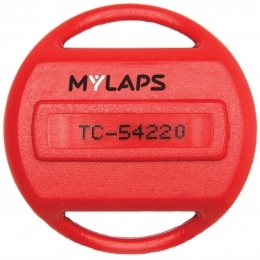
\includegraphics[width=4cm]{style/images/transponder}
  \end{center}
  \caption{MyLaps ProFlex transponder, op schaal}
  \label{fig:transponder}
  \vspace{15mm}
\end{wrapfigure}

In baansporten is de laatste jaren een ontwikkeling gaande om tijdregistratie te digitaliseren door het gebruik van transponders (bijvoorbeeld de MyLaps ProFlex transponder in Figuur~\ref{fig:transponder}) en detectie-lussen (Figuur~\ref{fig:detection-loop}) in de baan. Door deze ontwikkeling zijn nieuwe mogelijkheden ontstaan om ook naast het wedstrijdmoment de sportprestaties in te zien. Het constateren van de hierna genoemde nieuwe mogelijkheden was de aanleiding van dit project.

\begin{wrapfigure}{r}{4cm}
  \begin{center}
    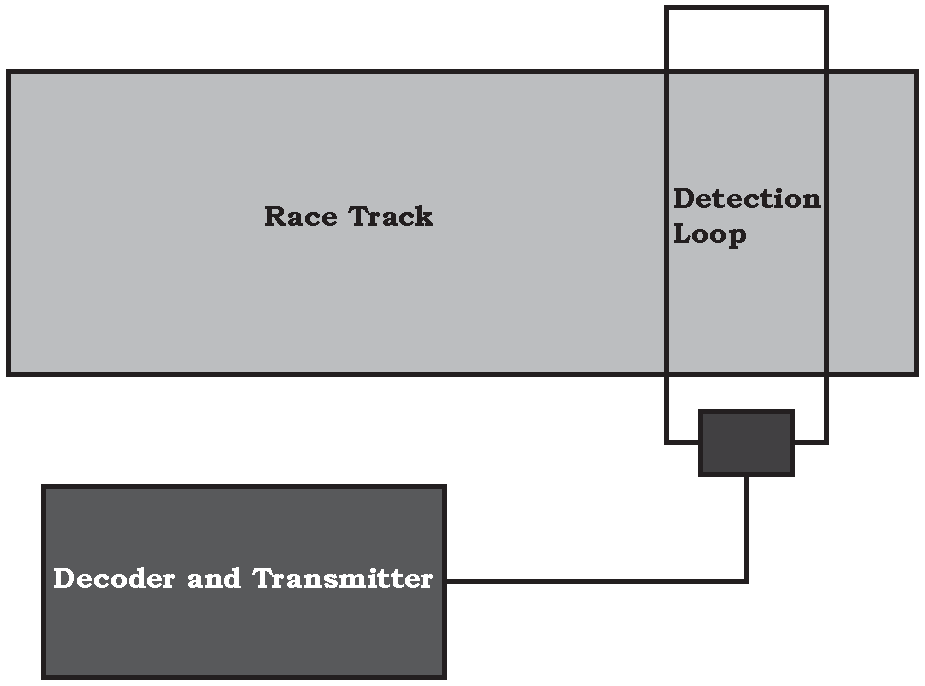
\includegraphics[width=4cm]{style/images/DetectionLoop}
  \end{center}
  \caption{Een schema van een detectielus en en decoder}
  \label{fig:detection-loop}
  \vspace{5mm}
\end{wrapfigure}

Een grote speler op de tijdregistratie-markt is MyLaps\footnote{\url{http://www.mylaps.com}}. Dit bedrijf installeert en beheert detectie-lussen en is actief bij diverse sporten zoals schaatsen, wielrennen, zwemmen, atletiek en diverse motorsporten. Bij sporten met permanente banen liggen de detectie-lussen het gehele jaar in de baan. Er bestaat de mogelijkheid om op de website van MyLaps doorkomst-tijden in te zien. De informatie die uit deze tijden is af te leiden, wordt door sporters als erg waardevol gezien om zich willen blijven verbeteren, waardoor er steeds meer getraind wordt met deze transponders.

\begin{figure}
  \begin{center}
    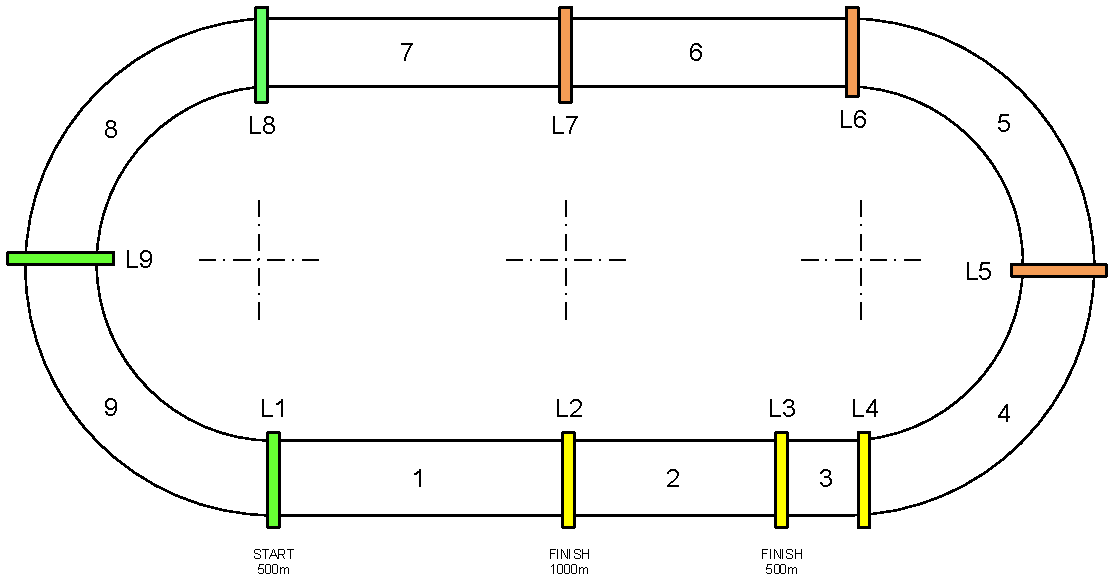
\includegraphics[width=0.8\textwidth]{style/images/BaanoverzichtHaarlem}
  \end{center}
  \caption{L1 tot en met L9 zijn de negen MyLaps transponderlussen in Haarlem}
  \label{fig:track-transponders}
\end{figure}

Voor aanvang van het seizoen worden door MyLaps detectielussen geïnstalleerd. De lussen bevinden zich in het ijs of onder het houten oppervlak van een baanwielrenbaan. Elke lus heeft een elektromagnetisch veld. Wanneer een sporter met transponder over dat veld heen rijdt, wordt de transponder geactiveerd en stuurt deze een unieke puls, die de lus opvangt. De MyLaps X2 server die aan de lussen zit aangesloten stuurt vervolgens het signaal door naar de MyLaps Cloud.

Het huidige gebruik van transponders - buiten wedstrijden - is voornamelijk achteraf, terwijl juist tijdens de training zowel sporter als coach het meeste bezig zijn met de prestaties. Het is daarom wenselijk om de resultaten in real-time door te geven aan coaches en sporters zelf.

Op veel banen zijn meerdere detectie-lussen geïnstalleerd, terwijl er op de website van MyLaps slechts één wordt ontsloten. In Thialf, de schaatsbaan in Heerenveen, Friesland, liggen bijvoorbeeld twaalf detectie-lussen, in Haarlem (Figuur~\ref{fig:track-transponders}) negen en op de andere schaatsbanen liggen er tenminste twee. Door de data van meerdere lussen te combineren is een betere indicatie te maken van de snelheid van sporters.

\begin{wrapfigure}{r}{0.4\textwidth}
 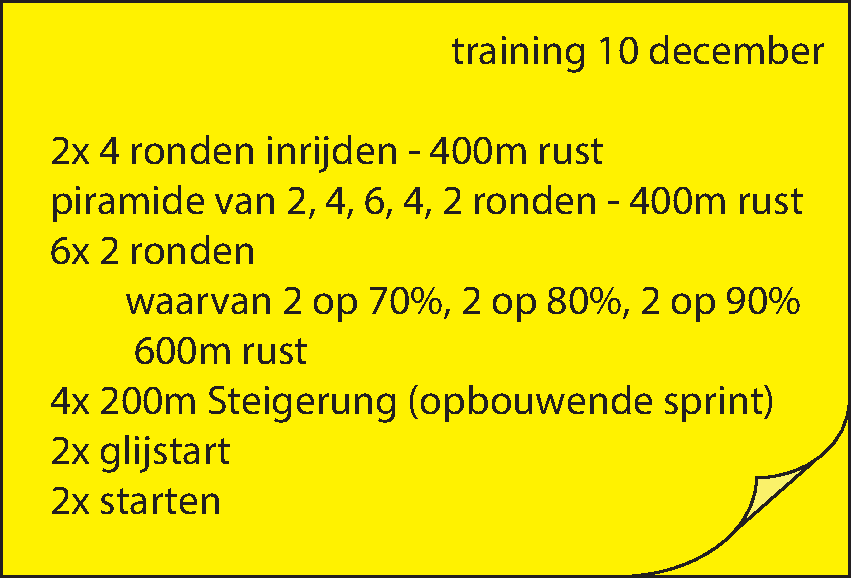
\includegraphics[width=0.4\textwidth]{style/images/training}
 \caption{Een typisch schaats-trainingsschema}
\end{wrapfigure}

Trainingen, bij bijvoorbeeld schaatsen, bestaan uit losse trainingsonderdelen. Allround schaatsers moeten bijvoorbeeld 4 ronden warmrijden, dan 6 keer 2 ronden sprinten, dan 4 keer een sprintje van 200 meter, 2 keer een glijstart en dan 2 keer een echte start bij de coach, vanuit de zijkant van de baan. Tussendoor is er rust, zo is het gebruikelijk om na een opdracht tenminste 400 meter uit te glijden. Het verschil tussen training en rust is af te leiden uit de verhouding tot de maximale snelheid.

Veel trainingselementen bestaan dus uit korte opdrachten, waar het juist om snelheid gaat. Een enkele lus is dan niet afdoende, omdat de rust voor of na de opdracht mee wordt gewogen. Sporters starten en stoppen namelijk niet precies boven de lus, maar starten vaak na de bocht en stoppen afhankelijk van de afstand van de opdracht op een willekeurig punt. 

Andere trainingen van bijvoorbeeld lange afstands- of marathonschaatsers kunnen bestaan uit één element: de hele training lang schaatsen, zonder overeind te komen. Wanneer er op tactische punten detectie-lussen geïnstalleerd zijn, is er bijvoorbeeld ook onderscheid te maken tussen bochten en de rechte stukken. Bij sporten met een ronde baan verschilt de snelheid in de bocht namelijk erg met die op het rechte eind. Deze vergelijking gebeurt nu al in Thialf, in het professionele circuit tijdens wedstrijden op televisie.

Topsporters zijn enorm prestatiegericht en als je al aan de top zit, dan kunnen kleine aanpassingen aan je techniek, ademhaling et cetera, grote verschillen maken. Coaches van professionele teams houden zich daarom bezig met allerhande analyses. Naast ademanalyse en hartslag monitoring, is het in Thialf bijvoorbeeld ook mogelijk om (van maximaal 20 schaatsers) continu de positie te bepalen met een in-door positioning system (IPS) ontwikkeld door InnoSportLab\footnote{\url{http://www.innosportlabthialf.nl}}.

Al deze geavanceerde analyses zijn echter te duur en kosten te veel tijd voor recreatieve sporters. MyLaps X2 biedt in combinatie met ons eindproduct recreatieve sporters toch een manier om analyses uit te voeren en zich naar een hoger niveau te tillen.

Aan de hand van de projectopdracht (zie de volgende sectie) en de gesprekken met Johan Stokking van Emando en onze TU-coach Cor-Paul Bezemer hebben we dit Plan van Aanpak opgesteld.

Dit Plan van Aanpak zal worden gebruikt als houvast bij het uitvoeren van dit project en wordt daarom ook goedgekeurd door alle betrokken partijen. Wanneer tijdens het project nieuwe inzichten worden opgedaan, kan het Plan van Aanpak in samenspraak met de betrokken partijen worden bijgesteld. Dit zal dan worden vermeld in voortgangsrapportages.

In dit document zal eerst de projectopdracht aan bod komen en zal worden toegelicht hoe deze tot stand is gekomen. Vervolgens wordt toegelicht op welke wijze we te werk zullen gaan en wat onze tijdsplanning is. Hierna wordt iets dieper ingegaan op de procesmatige inrichting van het project. Ten slotte zal er nog aandacht worden besteed aan kwaliteitsborging.

\section{Projectopdracht}
\subsection{Opdrachtomgeving}
Emando is een bedrijf dat zich momenteel onder andere richt op het ontwikkelen van Vantage. Een onderdeel van Vantage is een systeem voor tijdregistratie tijdens wedstrijden in baansporten. Een groot deel van de door Vantage gebruikte infrastructuur zou ook gebruikt kunnen worden voor de recreatieve- of amateurvariant van de sport. Hiervoor zou het project Trainingsapp voor Baansporten verschillende mogelijkheden moeten bieden.

\subsection{Doelstelling project}
Het project is bedoeld als pilot. Dit houdt in dat het een mogelijke toevoeging zou kunnen aan het bestaande Vantage platform, dat momenteel vooral gericht is op wedstrijden. Emando hoopt met dit project ook mogelijkheden te kunnen gaan bieden voor recreatieve sporters en voor trainingen.

\subsection{Opdrachtformulering}
In overleg met Emando is de projectopdract als volgt gedefinieerd:

\begin{quotation}
Het ontwerpen en ontwikkelen van een systeem voor het weergeven en analyseren van (live) recreatieve en trainingsdata in de context van baansporten (bijvoorbeeld schaatsen en baanwielrennen). Dit systeem zal realtime gegevens van de baan, maar ook opgeslagen gegevens uit het verleden, inzichtelijk maken voor sporters, coaches en eventuele toeschouwers (volgers). Daarnaast zal er de mogelijkheid zijn om een sociale component en een competitie element toe te voegen, en een mogelijkheid om aggregatie op data uit te voeren.

Het systeem ondersteunt het sporten: sporters hoeven hun training niet te onderbreken, doordat audio-cue's en sport-specifieke schermen geïmplementeerd worden. De sociale component bestaat uit het volgen van vrienden (mede-sporters) en het delen van resultaten. Het competitie element zal een virtuele competitie tussen vrienden omvatten.

Technisch gezien zal er een scheiding gemaakt worden tussen de diverse toepassingen (clients) en de API. De API biedt toegang tot realtime data en de diverse modulaire (sport-specifieke) aggregaties, waarbij de mogelijkheid bestaat voor bijvoorbeeld coaches om te abonneren op meerdere sporters. De API zal gekoppeld worden op bestaande systemen die data van transponders ontsluiten, en op databases met decennia aan historische sportresultaten van wedstrijden.
\end{quotation}

\subsection{Op te leveren producten en diensten}
Het project zal uiteindelijk resulteren in een product waarmee (live) recreatieve- en trainingsdata van baansporten wordt geanalyseerd en getoond aan sporters, coaches of toeschouwers. Verder zullen gedurende het project de volgende documenten worden opgeleverd: \begin{itemize}
\item Plan van Aanpak
\item Oriëntatie (onderdeel van verlag)
\item Programma van eisen (onderdeel van verslag)
\item Eindverslag
\item Reflectie aangaande de gang van het proces
\end{itemize}

\subsection{Specifieke producteisen}
De specifieke eisen aan dit project worden aangeduid met de sleutelwoorden “MOET” (MUST), “MAG NIET” (MUST NOT), “DIENT” (SHOULD) en “DIENT NIET” (SHOULD NOT). Deze sleutelwoorden komen overeen met de definities in RFC2119. De term “laten” kan worden opgevat als “in staat stellen tot”. Bij deze producteisen moet er rekening gehouden worden met het feit dat het hier gaat om een “minimum viable product” (MVP) en er een agile proces gebruikt wordt. Dit heeft tot gevolg dat de uiteindelijke implementatie hoogstwaarschijnlijk veel meer functionaliteit zal omvatten dan de hieronder genoemde punten en dat onderstaande requirements met grote waarschijnlijkheid aangepast/uitgebreid zullen worden.

Het product (MVP) dat opgeleverd wordt:
[bruikbaarheid]
MOET bruikbaar zijn als applicatie op smartphones
MOET bruikbaar zijn voor verschillende baansporten
[functionaliteit]
MOET op een ondersteunende manier inzicht geven in de presentaties van sporters. Daarom:
MOET het product real-time transponder doorkomsten van de sporter tonen en DIENT het deze te visualiseren
MOET het product historische gegevens van de sporter tonen en DIENT het deze te visualiseren
DIENT het product audio-cues te geven aan sporters
MOET een sociale component bevatten. Deze component:
MOET een gebruiker laten instellen wie toegang heeft tot zijn data
MOET een gebruiker zijn data laten delen met andere gebruikers
MOET een gebruiker data laten inzien die andere gebruikers met hem delen
DIENT een gebruiker competatief te laten interacteren met andere gebruikers
[beveiliging]
MAG NIET persoonsgegevens aan derden verstrekken zonder toestemming van de betreffende gebruiker
[technisch]
MOET real-time transponder doorkomsten met minimale vertraging verwerken
MOET een generieke API bevatten die ook gebruikt kan worden voor andere toepassingen
MOET een scheiding bevatten tussen de API (server) en de Client
MOET een koppeling hebben met bestaande infrastructuren voor het ontsluiten van transpondergegevens en historische data
Specifieke proceseisen
Gedurende het project zal er per teamlid 40 uur per week gewerkt worden aan het project, zoals overeen gekomen in de stageovereenkomst.
De projectwerkzaamheden zullen voor het grootste deel plaatsvinden op het kantoor van Emando te Amsterdam. 
De opdrachtgever zal ervoor zorgen dat de teamleden een werkplek hebben wanneer zij hun werkzaamheden uitvoeren op het kantoor van Emando.
Om goed contact met de TU-coach te behouden, zal er tevens gewerkt worden op de Technische Universiteit Delft.
Het ontwikkelproces zal agile zijn. Dat wil zeggen dat de requirements in dit document later in het proces aangepast kunnen (en zullen) worden in samenspraak tussen het team en de opdrachtgever. Daarnaast zal het product worden opgeleverd in verschillende iteraties, waarin telkens functionaliteit aan het product wordt toegevoegd.
Er zal gewerkt worden met de “minimum viable product”-aanpak (MVP). Dat wil zeggen dat er in eerste instantie een product moet worden opgeleverd met precies de kernfunctionaliteiten en niet meer. In een later stadium kan er op een iteratieve manier extra functionaliteit toegevoegd worden.
De teamleden zullen zorg uitdragen om de projectwerkzaamheden naar beste weten en kunnen uit te voeren. Daarbij worden echter geen garanties gedaan over de verwachte resultaten, zoals deze omschreven zijn in de opdracht.

\section{Tijdsplanning}
Iedere week zal er gefocust worden op bepaalde aspecten en functionaliteiten. De planning is opgenomen als Appendix~\ref{ch:planning}.

\section{Projectinrichting}

\subsection{Proces}
Naast de aspecten uit de tijdsplanning zullen we elke werkdag beginnen met een stand-up: elk teamlid vertelt gedurende maximaal een tien minuten wat hij afgelopen dag bereikt heeft en wat hij van plan is die dag te doen. De opdrachtgever heeft aangegeven hier zo vaak als voor hem mogelijk is bij aanwezig te zijn. Aan het eind van elke week is er een demo.

De voortgang van het proces zal worden bijgehouden door middel van een issue tracker en een (digitaal) SCRUM~\cite{scrum} bord. De teamleden zullen met behulp van deze tools de voortgang van het proces inzichtelijk maken en een overzicht kunnen geven van het project.

Zoals per stagecontract afgesproken, zal er per teamlid 40 uur per week gewerkt worden aan het project, waarbij teamleden zorg zullen uitdragen om de projectwerkzaamheden naar beste weten en kunnen uit te voeren. Er is in die zin een gedeelde verantwoordelijkheid, waar teamleden elkaar zonodig bijsturing geven. 

\subsection{Resources}
De opdrachtgever stelt gedurende de periode van 1 mei tot het eind van het project een werkplek ter beschikking in het kantoor aan het Leidseplein in Amsterdam. We zullen gedurende het project op onze eigen laptops werken. Via AcademicDownload\footnote{\url{http://academicdownload.com}} verschaft de TU Delft studenten licenties voor Windows 8.1 Enterprise. Overige licenties voor ontwikkeltools zullen door de opdrachtgever worden verzorgd.

Via MyLaps zal de opdrachtgever ons toegang verschaffen tot de transponder-data. Overige data van onder andere de KNSB zal ook via het netwerk van de opdrachtgever worden verkregen.

\section{Kwaliteitsborging}
De opdrachtgever houdt via het SCRUM bord de voortgang in de gaten en zal bij dagelijkse stand-ups de voortgang kunnen controleren.  In het laatste hoofdstuk wordt uitgewerkt op welke wijze de opdrachtgever en de projectleden in staat zijn de kwaliteit van het project te beïnvloeden. Hoewel harde voorwaarden in hoofdstuk 2 zijn verwoord, wordt hier verder uitgewerkt wat met name de opdrachtgever kan doen om bij te dragen aan een hoge kwaliteit.

Als laatste worden de maatregelen beschreven die beide partijen zullen treffen om bekende risico’s te voorkomen.

\section{Bijlagen}

Eventuele bijlagen waarnaar verwezen wordt zullen hier worden opgenomen. Notulen van eerder gevoerde gesprekken behoren tot deze documenten.